\section{Applications}\label{sec:app}
The integrated gradients technique
is applicable to a variety of deep networks. Here, we
apply it to two image models, two natural language
models, and a chemistry model.

\subsection{An Object Recognition Network}\label{sec:app-incp}
We study feature attribution in an object recognition network built
using the GoogleNet architecture~\cite{SLJSRAEVR14} and trained over
the ImageNet object recognition dataset~\cite{ILSVRC15}.
%% It is $22$
%% layers deep with a softmax layer on top for
%% classifying images into one of the $1000$ ImageNet object classes.
%% The input to the network is a $224 \times 224$ sized RGB image.
We use the integrated gradients method to study pixel importance in
predictions made by this network. The gradients are computed for the
output of the highest-scoring class with respect to pixel of the input
image. The baseline input is the black image, i.e., all pixel intensities
are zero.
%% Integrated gradients essentially aggregate the gradients of
%% images obtained by interpolating between the original image and this
%% black image.

Integrated gradients can be visualized by aggregating them along the
color channel and scaling the pixels in the actual image by them.
Figure~\ref{fig:intgrad-finalgrad} shows visualizations for a
bunch of images\footnote{More examples can be found at
  \url{https://github.com/ankurtaly/Attributions}}.  For comparison,
it also presents the corresponding visualization obtained from the
product of the image with the gradients at the actual image.
Notice that integrated gradients are better at reflecting distinctive
features of the input image.

%% To further quantify the effectiveness
%% of integrated gradients over gradients, we perform two analyses.
%% \begin{enumerate}
%% \item \textbf{Pixel ablations:} Based on a method proposed
%%   by~\cite{SBMBM15}, we ablate (i.e, zero the pixel intensity) the top
%%   $5000$ pixels ($10\%$ of the image) by attribution, and compute the
%%   score drop for the highest scoring object class. We find that
%%   ablating the top pixels identified by integrated gradients leads to
%%   a larger score drop that those identified by gradients at the image
%%   for $132$ out of $150$ randomly chosen images.
%% \item \textbf{Localization:} We consider images from the 2012 ImageNet
%%   object localization dataset with human-drawn bounding boxes around objects,
%%   and compute the percentage of pixel attribution inside the bounding box.
%%   We run our evaluation over $100$ randomly chosen
%%   images and find that on $82$ images the integrated gradients technique
%%   leads to a higher fraction of the pixel attribution inside the box than
%%   gradients at the actual image. The average difference in the percentage
%%   pixel attribution inside the box for the two techniques is $8.4\%$.
%% \end{enumerate}

\begin{figure}[!htb]
  \centering
  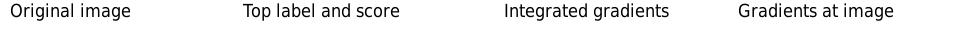
\includegraphics[width=0.7\columnwidth]{./Figures/IntegratedGrads/img0.jpg}
  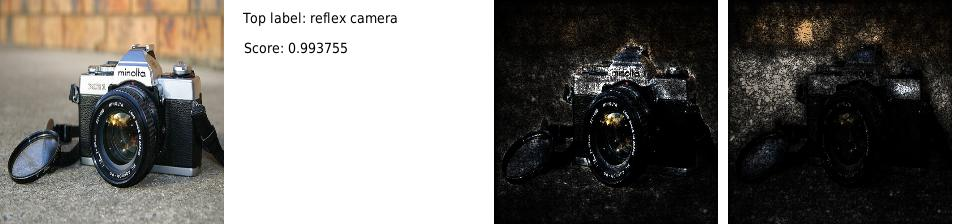
\includegraphics[width=0.7\columnwidth]{./Figures/IntegratedGrads/img1.jpg}
  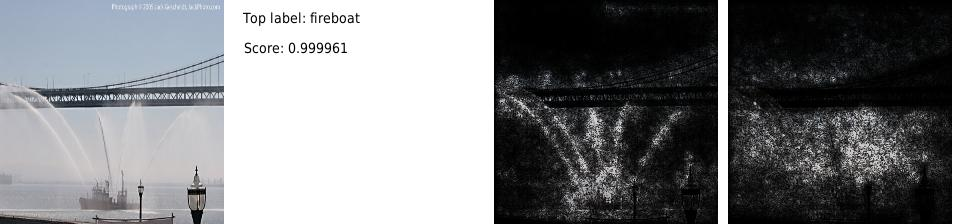
\includegraphics[width=0.7\columnwidth]{./Figures/IntegratedGrads/img2.jpg}
  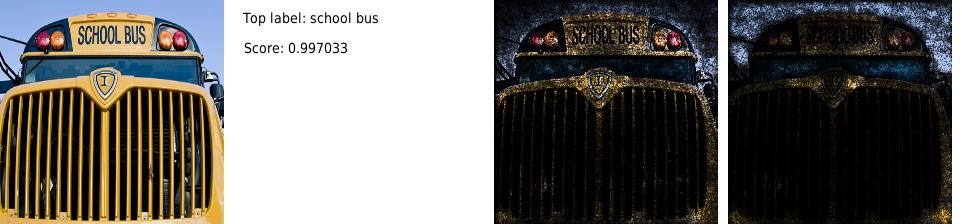
\includegraphics[width=0.7\columnwidth]{./Figures/IntegratedGrads/img3.jpg}
  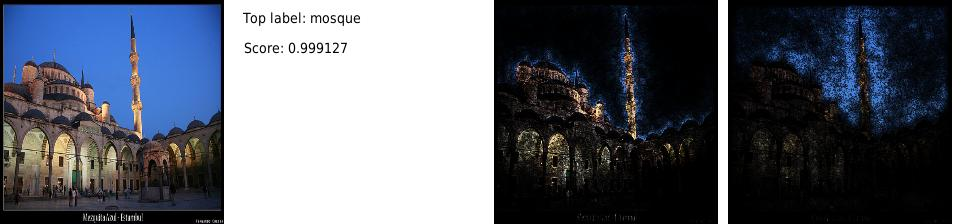
\includegraphics[width=0.7\columnwidth]{./Figures/IntegratedGrads/img4.jpg}
  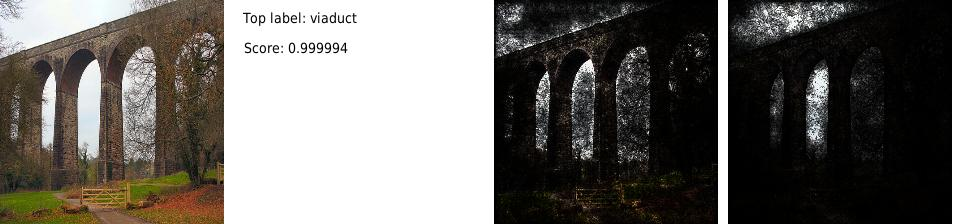
\includegraphics[width=0.7\columnwidth]{./Figures/IntegratedGrads/img5.jpg}
  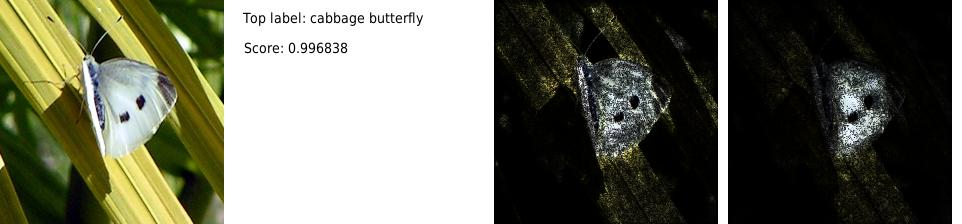
\includegraphics[width=0.7\columnwidth]{./Figures/IntegratedGrads/img6.jpg}
  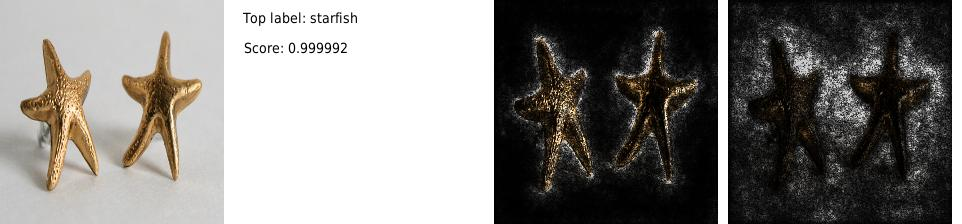
\includegraphics[width=0.7\columnwidth]{./Figures/IntegratedGrads/img7.jpg}
  \caption{\textbf{Comparing integrated gradients with gradients at the image.}
    Left-to-right: original input image, label and softmax score for
    the highest scoring class, visualization of integrated gradients,
    visualization of gradients*image.
    Notice that the visualizations
    obtained from integrated gradients are better at reflecting distinctive
    features of the image.
  }\label{fig:intgrad-finalgrad}
\end{figure}

%% \begin{figure}[!htb]
%%   \centering
%%   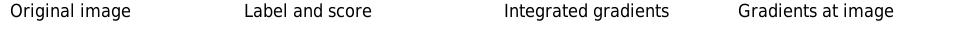
\includegraphics[width=0.7\columnwidth]{./Figures/IntegratedGradsOverlayVis/title.jpg}
%%   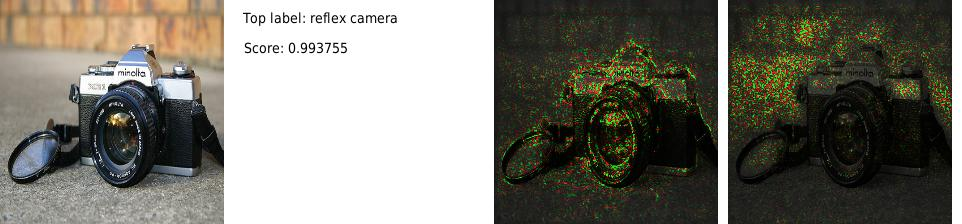
\includegraphics[width=0.7\columnwidth]{./Figures/IntegratedGradsOverlayVis/8e570672510267d3.jpg}
%%   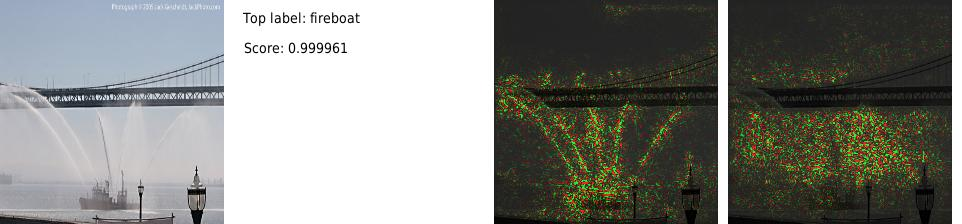
\includegraphics[width=0.7\columnwidth]{./Figures/IntegratedGradsOverlayVis/70bfca4555cca92e.jpg}
%%   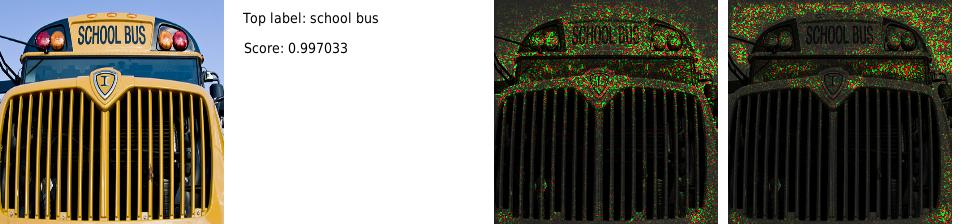
\includegraphics[width=0.7\columnwidth]{./Figures/IntegratedGradsOverlayVis/700a04c5c2ca6e80.jpg}
%%   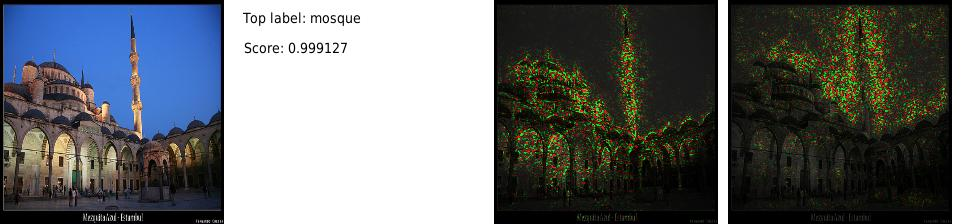
\includegraphics[width=0.7\columnwidth]{./Figures/IntegratedGradsOverlayVis/80c64f2e27f8784a.jpg}
%%   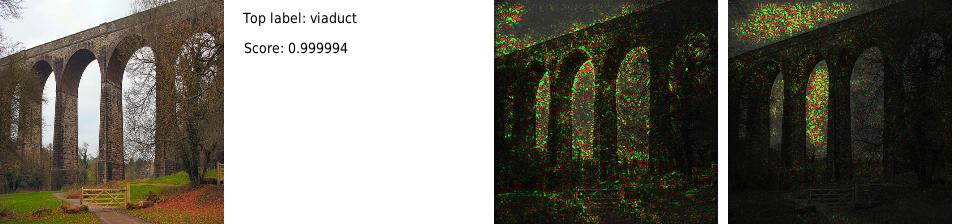
\includegraphics[width=0.7\columnwidth]{./Figures/IntegratedGradsOverlayVis/c0a9ce885a9c26bc.jpg}
%%   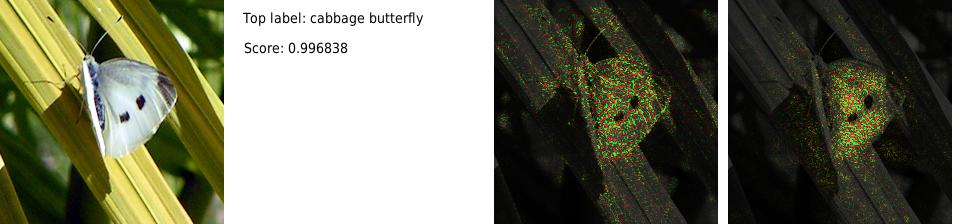
\includegraphics[width=0.7\columnwidth]{./Figures/IntegratedGradsOverlayVis/1bd6987fa9219dec.jpg}
%%   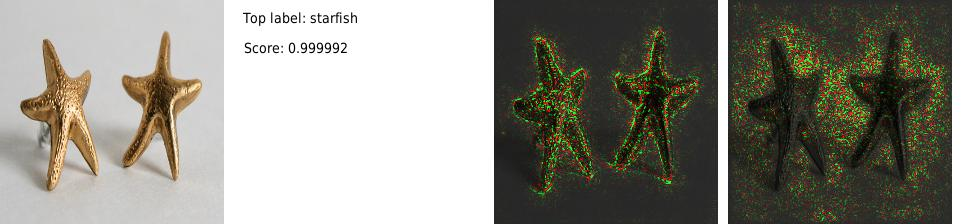
\includegraphics[width=0.7\columnwidth]{./Figures/IntegratedGradsOverlayVis/2587b0bd7d764bd9.jpg}
%%   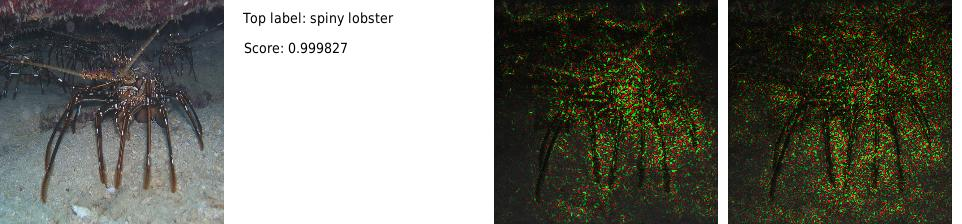
\includegraphics[width=0.7\columnwidth]{./Figures/IntegratedGradsOverlayVis/a2c980be2b5d464d.jpg}
%%   \caption{\textbf{Comparing integrated gradients with gradients at the image.}
%%     Left-to-right: original input image, label and softmax score for
%%     the highest scoring class, visualization of integrated gradients,
%%     visualization of gradients at the image. Notice that the visualizations
%%     obtained from integrated gradients are better at reflecting distinctive
%%     features of the image.}\label{fig:intgrad-finalgrad}
%% \end{figure}


\subsection{Diabetic Retinopathy Prediction}\label{sec:app-dr}

Diabetic retinopathy (DR) is a complication of the diabetes that
affects the eyes. Recently, a deep network~\cite{jama-dr} has been proposed
to predict the severity grade for DR in retinal fundus images. The model has
good predictive accuracy on various validation datasets.

We use integrated gradients to study feature importance for this
network; like in the object recognition case, the baseline is the
black image.
Feature importance explanations are important for this network
as retina specialists may use it to
build trust in the network's predictions, decide the grade for
borderline cases, and obtain insights for further testing and
screening.
%% Feature importance explanations are important for this network
%% as surfacing them to retina specialists helps to
%% encourage clinical adoption.
%% Retina specialists may use it to
%% build trust in the network's predictions, decide the grade for
%% borderline cases, and obtain insights for further testing and
%% screening.

Figure~\ref{fig:dr} shows a visualization of integrated gradients for
a retinal fundus image. The visualization method is a bit different
from that used in Figure~\ref{fig:intgrad-finalgrad}.
We aggregate integrated gradients along the color channel and
overlay them on the actual image in gray scale with positive
attribtutions along the green channel and negative attributions
along the red channel.
Notice that integrated gradients are localized
to a few pixels that seem to be lesions in the retina. The interior of
the lesions receive a negative attribution while the periphery receives
a positive attribution indicating that the network focusses on the
boundary of the lesion.

%% We evaluated integrated gradients as part of wider study with retina
%% specialists and found that integrated gradients help the
%% specialist confirm the predicted DR grade on $28$ out of $33$ images
%% from the EyePACs-1 dataset~\cite{jama-dr} chosen for diversity. We are
%% currently scaling this study.

\begin{figure}[!htb]
  \centering
  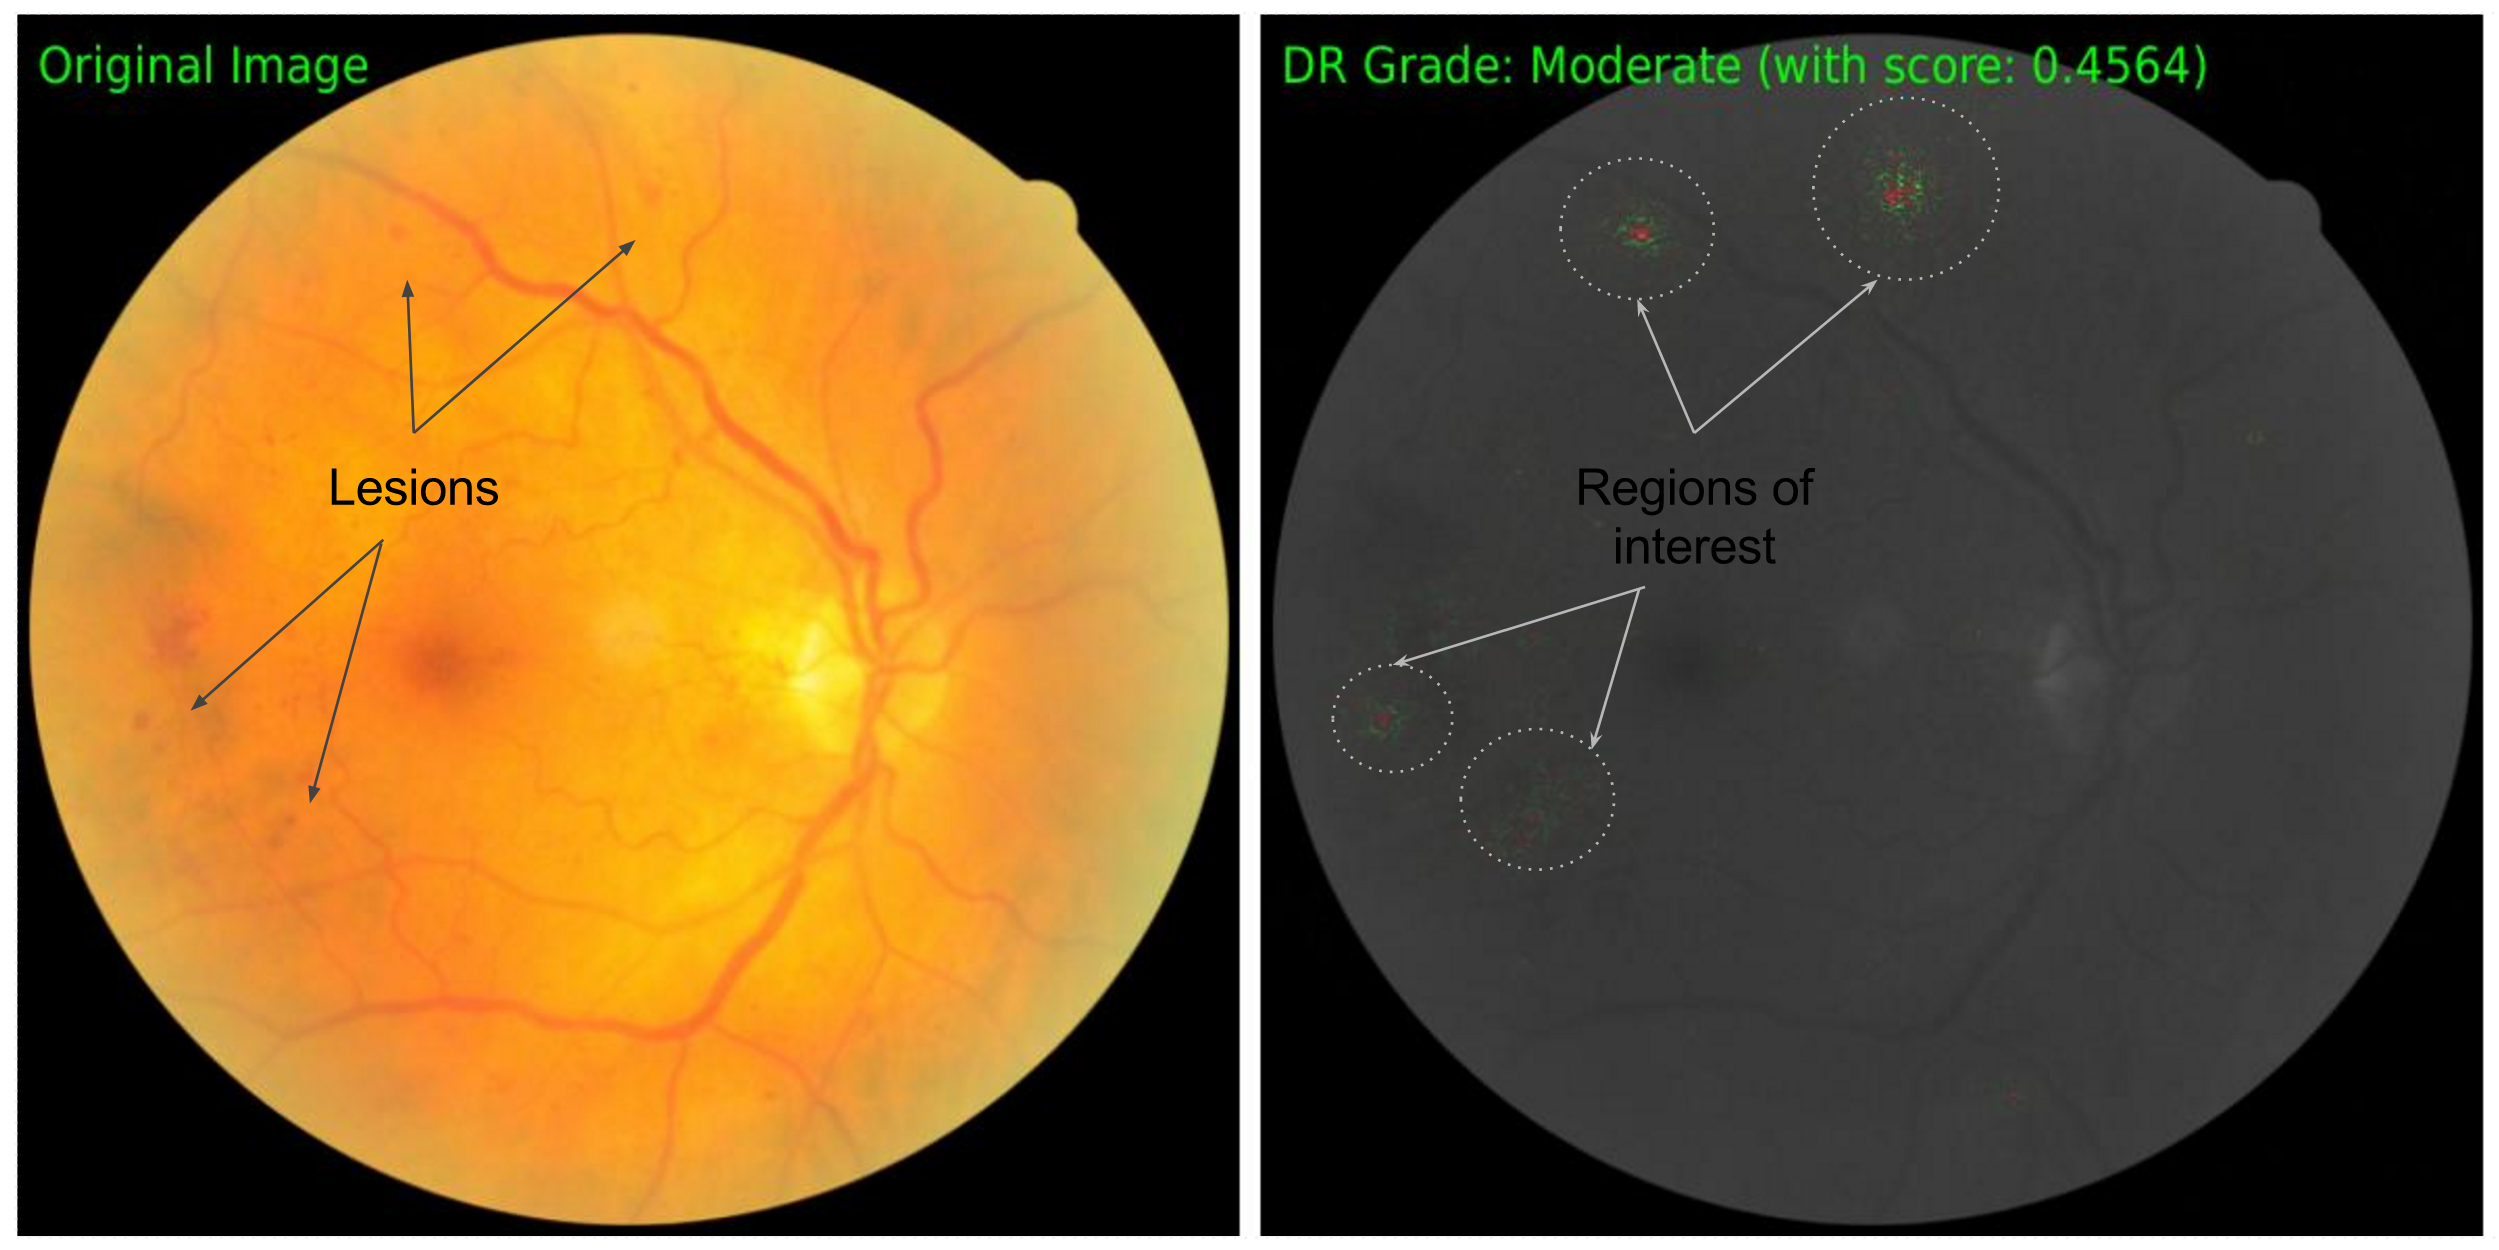
\includegraphics[width=0.8\columnwidth]{./Figures/Retina/retina_with_red.png}
  \caption{\textbf{Attribution for Diabetic Retinopathy grade prediction from a retinal fundus image.}
    The original image is show on the left, and the attributions (overlayed on the
    original image in gray scaee) is shown on the right. On the original image we annotate
    lesions visible to a human, and confirm that the attributions indeed point to them.}\label{fig:dr}
\end{figure}


\subsection{Question Classification}\label{sec:app-qc}
Automatically answering natural language questions (over
semi-structured data) is an important problem in artificial
intelligence (AI).  A common approach is to semantically parse the
question to its logical form~\cite{L16} using a set of
human-authored grammar rules. An alternative approach is to machine
learn an end-to-end model provided there is enough training data.
%% Rule based systems have the advantage of being more precise at language
%% understanding~\cite{L16}, more maintainable and easy to debug. The
%% downside is that they have poorer recall. This is because there are
%% often multiple phrasing of the same question in natural language,
%% e.g., ``how many people work at Walmart?'' and ``what is the number of
%% employees at Walmart?''  It is hard for human-authored rules to be
%% comprehensive on all possible phrasings. This is
%% where machine learnt models are better.
An interesting question is whether one could peek inside
machine learnt models to derive new rules.
%% for improving recall of the
%% overall system.
We explore this direction for a sub-problem of
semantic parsing, called \textbf{question classification}, using the
method of integrated gradients.

The goal of question classification is to identify the
type of answer it is seeking. For instance, is
the quesiton seeking a yes/no answer, or is it seeking a date? Rules
for solving this problem look for trigger phrases in the question, for
e.g., a ``when'' in the beginning indicates a date seeking
question.
We train a model for question classification using the
the text categorization architecture
proposed by~\cite{K14} over the WikiTableQuestions dataset~\cite{PL15}.
We use integrated gradients to attribute
predictions down to the question terms in order to identify new
trigger phrases for answer type.
The baseline input is the all zero embedding vector.

Figure~\ref{fig:qc} lists a few questions with constituent terms
highlighted based on their attribution.  Notice that the attributions
largely agree with commonly used rules, for e.g., ``how many''
indicates a numeric seeking question. In addition, attributions
help identify novel question classification rules, for e.g.,
questions containing ``total number'' are seeking numeric answers.
Attributions also point out undesirable correlations, for e.g.,
``charles'' is used as trigger for a yes/no question.

\begin{figure}[!htb]
  \centering
  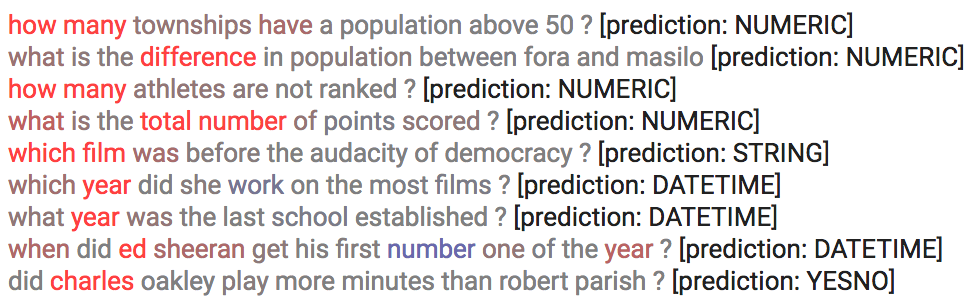
\includegraphics[width=\columnwidth]{./Figures/QuestionClassification/attributions.png}
  \caption{\textbf{Attributions from question classification model.} Term color indicates attribution
    strength---Red is positive, Blue is negative, and Gray is neutral (zero). The predicted
    class is specified in square brackets.}
  \label{fig:qc}
\end{figure}

\subsection{Neural Machine Translation}\label{sec:app-nmt}
We applied our technique to a complex, LSTM-based Neural Machine Translation System~\cite{Wu16}.
We attribute the output probability of every output token (in form of wordpieces)
to the input tokens. Such attributions ``align'' the output sentence with the input sentence.
For baseline, we zero out the embeddings of all tokens except the start and end markers.
Figure~\ref{fig:nmt} shows an example of such an attribution-based alignments.
We observed that the results make intuitive sense. E.g. ``und'' is mostly attributed to ``and'',
and ``morgen'' is mostly attributed to ``morning''.
We use $100-1000$ steps (cf. Section~\ref{sec:applying}) in the integrated gradient approximation; we need this because the network is highly nonlinear.

\begin{figure}[!htb]
  \centering
  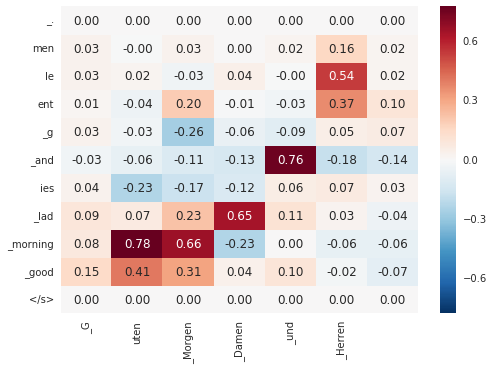
\includegraphics[width=0.7\columnwidth]{./Figures/NMT/nmt.png}
  \caption{\textbf{Attributions from a language translation model.} Input in English: ``good morning ladies and gentlemen''. Output in German: ``Guten Morgen Damen und Herren''. Both input and output are tokenized into word pieces, where a word piece prefixed by underscore indicates that it should be the prefix of a word.}
  \label{fig:nmt}
\end{figure}

%\subsection{Penn Treebank model}\label{sec:app-ptb}
%We apply our technique to word-level language modeling of the Penn
%Treebank dataset~\cite{MSM94}, and apply an LSTM-based sequence model
%based on~\cite{ZSV14}. For such a network, given a sequence of input words,
%and the softmax prediction for the next word, we want to identify the importance
%of the preceding words.
%
%To describe the setup, we choose 20 randomly chosen sections of the test data,
%and for each of them inspect the prediction score of the next word using the
%first $10$ words. The baseline here is obtained by zeroing out the embedding
%vectors, just as in the question classification model.
%% \begin{figure*}[!htb]
%%   \footnotesize
%% \begin{center}
%%   \begin{tabular}{ | l | c c c c c  r |}
%%     \hline
%%     Sentence & the & shareholders & claimed & more & \textbf{than} & \$ N millions in losses \\ \hline
%%     Integrated gradients & -0.1814& -0.1363 & 0.1890& {\bf 0.6609} &  &  \\ 
%%     Gradients & 0.0007 & -0.0021 & 0.0054 & -0.0009 &  &  \\ \hline
%%   \end{tabular}
%% \end{center}
%% \caption{Prediction for \textbf{than}: 0.5307, total integrated gradient: 0.5322}
%% \label{tab:ptb_near}
%% \end{figure*}

%% \begin{figure*}[!htb]
%%   \scriptsize
%%   \begin{center}
%%     \scriptsize
%%   \begin{tabular}{ | l | c c c c c c r |}
%%     \hline
%%     Sentence               & and       & N   & minutes  & after  &   the    & ual    & trading  \\ \hline
%%     Integrated gradients (*1e-3) & 0.0707&0.1286& 0.3619& 1.9796& -0.0063& {\bf 4.1565}& 0.2213\\ 
%%     Gradients (*1e-3)          & 0.0066& 0.0009& 0.0075& 0.0678& 0.0033& 0.0474& 0.0184 \\ \hline
%%     Sentence (Cont.)       & halt      & came      & news      &that       &the        &\textbf{ual}& group  \\ \hline
%%     Integrated gradients (*1e-3) & -0.8501& -0.4271& 0.4401& -0.0919& 0.3042 &  &  \\ 
%%     Gradients (*1e-3) & -0.0590 &  -0.0059& 0.0511& 0.0041&0.0349 &  &  \\ \hline
%%   \end{tabular}
%% \end{center}
%% \caption{Prediction for \textbf{ual}: 0.0062, total integrated gradient: 0.0063}
%% \label{tab:ptb_far}
%% \end{figure*}

%% In Table~\ref{tab:ptb_far} we show a
%% comparisons of integrated gradients to gradients.  Due to saturation,
%% the magnitudes of gradients are so small compared to the prediction
%% scores that it is difficult to make sense of them.  In comparison,
%% integrated gradients have a total amount close to the
%% prediction, and seem to make sense.
%% %% For example, in the first example,
%% %% the integrated gradients attribute the prediction score of ``than`` to
%% %% the preceding word ``more''.
%% %% This makes sense as ``than'' often
%% %% follows right after ``more`` in English.  On the other hand, standard
%% %% gradient gives a slightly negative attribution that betrays our
%% %% intuition.
%% In the example, in predicting the second ``ual'',
%% integrated gradients are clearly the highest for the first occurrence
%% of ``ual'', which is the only word that is highly predictive of the
%% second ``ual''.

%% In
%% contrast, our method is extremely easy to implement, and is faithful
%% to the original network at least in offering an exact attribution of
%% the network's output to the input features.

\subsection{Chemistry Models}\label{sec:app-chem}
We apply integrated gradients to a network performing Ligand-Based
Virtual Screening which is the problem of predicting whether an input
molecule is active against a certain target (e.g., protein or enzyme).
In particular, we consider a network based on the molecular graph
convolution architecture proposed by~\cite{KMBPR16}.
%% Understanding
%% feature importance in molecules predicted to be active against may
%% help medicinal chemists in identifying the dominant molecular
%% substructures--- formally, \emph{pharmacophores}---that are
%% responsible for the activity. It may also help sanity check the
%% behavior of the network---we discuss an anecdote about this later in
%% this section.

The network requires an input
molecule to be encoded by hand as a set of atom and atom-pair features
describing the molecule as an undirected graph. Atoms are featurized
using a one-hot encoding specifying the atom type (e.g., C, O, S,
etc.), and atom-pairs are featurized by specifying either the type of
bond (e.g., single, double, triple, etc.)  between the atoms, or the
graph distance between them.
%% \footnote{This featurization is referred to as ``simple'' input featurization
%%   in~\cite{KMBPR16}.}
The baseline input is obtained zeroing out the feature vectors for
atom and atom-pairs.

%% The careful reader might notice that these counterfactual inputs are
%% not valid featurizations of molecules. However, we argue that they are
%% still valid inputs for the network. First, all operators in the
%% network (e.g., ReLUs, Linear filters, etc.) treat their inputs as
%% continuous real numbers rather than discrete zeros and ones. Second,
%% all fields of the counterfactual inputs are bounded between zero and
%% one, therefore, we don't expect them to appear spurious to the
%% network. We discuss this further in section~\ref{sec:discussion}

We visualize integrated gradients as heatmaps over the the atom and
atom-pair features with the heatmap intensity depicting the strength
of the contribution. Figure~\ref{fig:attribution-gas} shows the
visualization for a specific molecule. Since integrated gradients add
up to the final prediction score (see
Proposition~\ref{prop:additivity}), the magnitudes can be use for
accounting the contributions of each feature.  For instance, for the
molecule in the figure, atom-pairs that have a bond between them
cumulatively contribute to $46\%$ of the prediction score, while all
other pairs cumulatively contribute to only $-3\%$.

%% We presented the attributions for $100$ molecules active against a
%% specific task to a few chemists. The chemists were able to immediately
%% spot dominant functional groups (e.g., aromatic rings) being surfaced
%% by the attributions.
%% A next step could be cluster the aggregate the
%% attributions across a large set of molecules active against a specific
%% task to identify a common denominator of features shared by all active
%% molecules.

\begin{figure}[!ht]
  \centering
  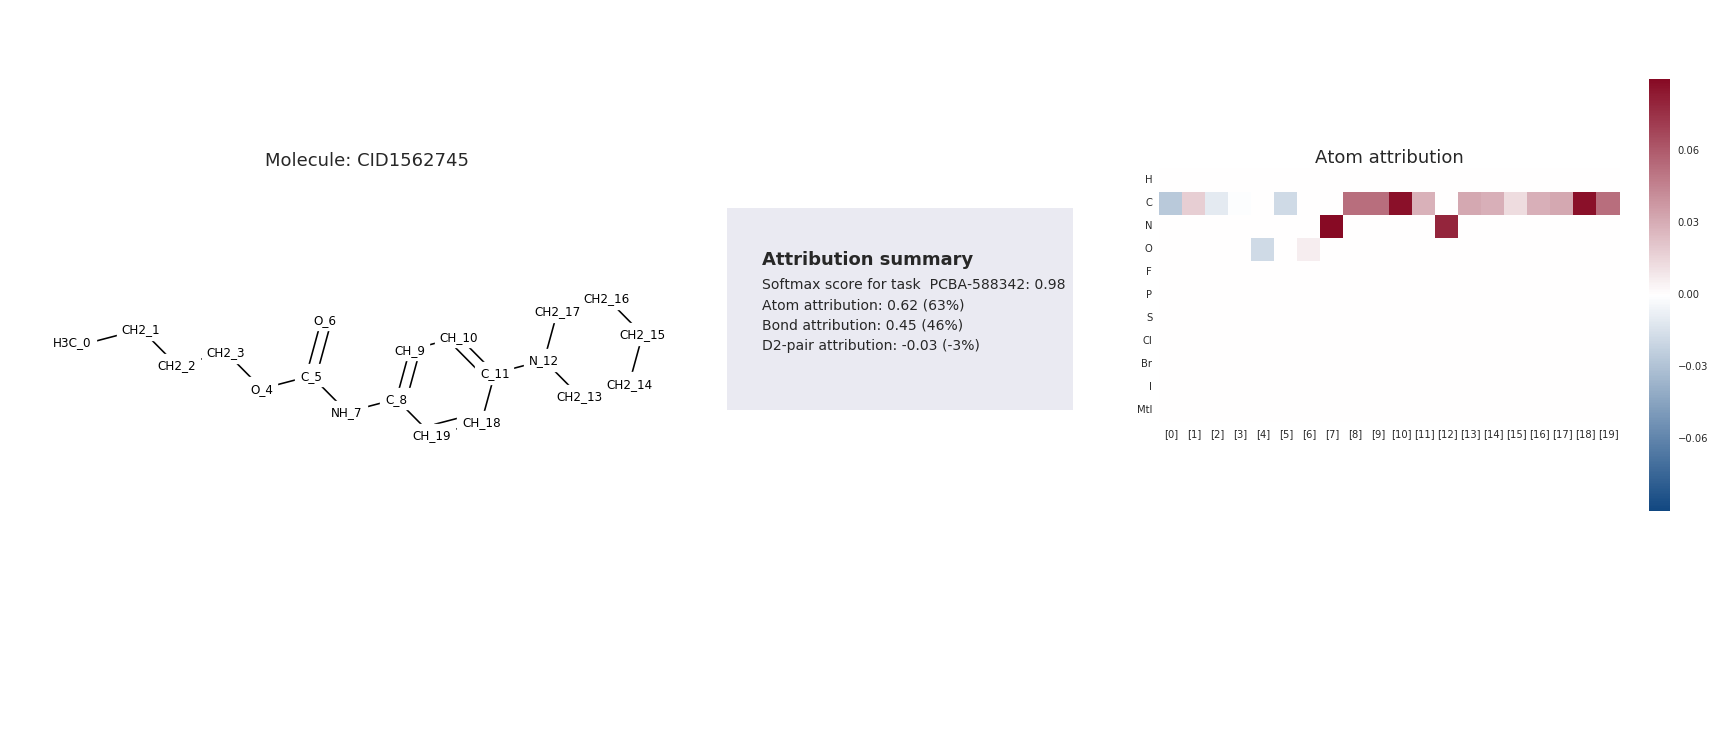
\includegraphics[width=0.9\columnwidth]{./Figures/GAS/W2OneHot/attr-vis-atoms.png}
  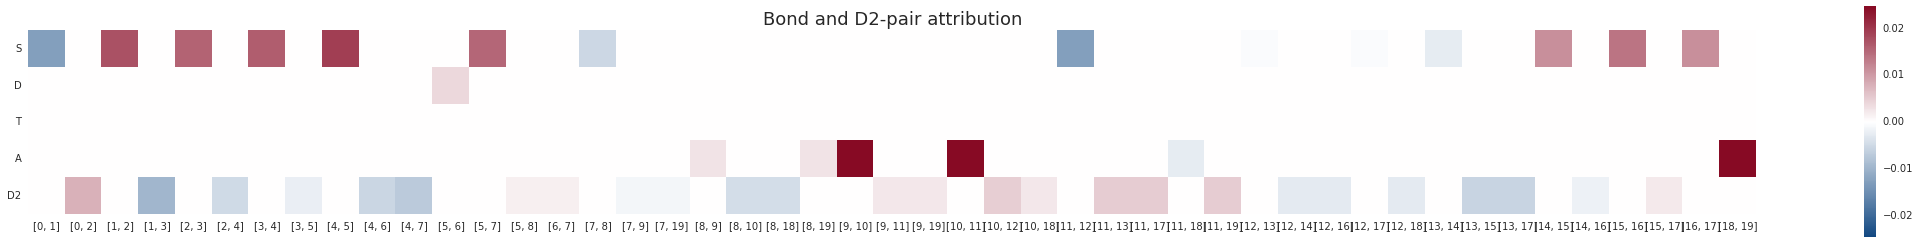
\includegraphics[width=0.9\columnwidth]{./Figures/GAS/W2OneHot/attr-vis-pairs.png}
  \caption{\textbf{Attribution for a molecule under the W2N2 network~\cite{KMBPR16}}.
    The molecules is active on task PCBA-58432.}\label{fig:attribution-gas}
\end{figure}

\stitle{Identifying Degenerate Features}
We now discuss how attributions helped us spot an anomaly in the W1N2
architecture in ~\cite{KMBPR16}. On applying the integrated gradients
method to this network, we found that several atoms in the same
molecule received identical attribution despite being bonded to
different atoms. This is surprising as one would expect two atoms with
different neighborhoods to be treated differently by the network.

On investigating the problem further, in the network architecture,
the atoms and atom-pair features were not fully convolved. This
caused all atoms that have the
same atom type, and same number of bonds of each type to contribute
identically to the network.

%% Despite the aforementioned problem, the W1N2 network had good
%% predictive accuracy. One hypothesis for this is that the atom type and
%% their neighborhoods are tightly correlated; for instance an outgoing
%% double bond from a Carbon is always to another Carbon or Oxygen
%% atom. As a result, given the atom type, an explicit encoding of the
%% neighborhood is not needed by the network. This also suggests that
%% equivalent predictive accuracy can be achieved using a simpler ``bag
%% of atoms'' type model.




